\documentclass{article}
% \documentclass[UTF8]{ctexart}
\usepackage{amsmath,amssymb,amsfonts}  % For math symbols and fonts
\usepackage{graphicx}                   % For including images
\usepackage{hyperref}                   % For hyperlinks
\usepackage{cite}                       % For citations
% \usepackage[UTF8]{ctex}  % 注意,不是 \documentclass[UTF8]{ctexart}
% \renewcommand{\contentsname}{Contents}
% \renewcommand{\refname}{References}
% \renewcommand{\abstractname}{Abstract}

\usepackage{algorithm}
\usepackage{algorithmic}

\usepackage{amsthm}
% Define new theorem-like environments
% Define environments
\theoremstyle{definition} % Non-italicized style
\newtheorem{definition}{Definition}[section]
\newtheorem{exercise}{Exercise}[section]

% Title and author info
\title{Wavelet Transform for Image Processing}
\author{
Zhang Jinrui\thanks{alternative email:zhangjr1022@mails.jlu.edu.cn} \\ \texttt{jerryzhang40@gmail.com}
}

\date{20250728}  % Empty date; optional, you can also specify a date here

\begin{document}

\maketitle

\begin{abstract}
    In this article, I tried to use
    Wavelet Transform to compress
    images.
\end{abstract}


\section{Decomposition \& Mother Wavelet}
A mother wavelet \(\psi\) satisfied
following property.
\(\langle\psi,\psi\rangle=1\)

And the family of the Hilbert Basis
wavelets are as follow.
\[
    \psi_{j,k}=\sqrt{2^j}\psi(2^j(x-2^{-j}k)) \, j,k\in \mathbb{Z}
\]

A function \(f\) can be decomposed
use these basis as follow.

\[
    f=c_{j,k}\psi_{j,k}
\]

There are 10 drones and fly on the sky
obeys Newton's second law of motion.
which is
\[
    \vec{F} = m \vec{a}
\]
\[
    \vec{a} = \frac{d\vec{v}}{dt} = \frac{d^2 \vec{x}}{dt^2}
\]
And I mean the policy by, we need a function of force
depending on some communication between drones
to decide the \(\vec{F}\)
\[
    \vec{F}=f(the current information)
\]

And then we want the following dynamic system
\[\begin{bmatrix}
        \frac{d\vec{d}}{dt} \\
        \frac{d\vec{v}}{dt}
    \end{bmatrix}=
    \begin{bmatrix}
        \vec{v} \\
        \vec{a}=f/m
    \end{bmatrix}
\]
has some Self-organized emergent phenomena,
to automatically emergent a circle rounding pattern.

question: framelet multiresolution(sacle function and funciont)

\section{Haar 1D sequence Decomposition}
For a \(2^{N}\) points sequence, the mother
wavelet is
\[
    \psi(n) =
    \begin{cases}
        0,                     & \text{if } n < 0               \\
        \frac{1}{\sqrt{2^N}},  & \text{if } 0\leq n < 2^{N-1}   \\
        \frac{-1}{\sqrt{2^N}}, & \text{if } 2^{N-1}\leq n<2^{N} \\
        0,                     & \text{if } n >= 2^N            \\
    \end{cases}
\]
We have
\[
    \langle\psi,\psi\rangle=\sum_{k=0}^{2^N-1}\frac{1}{2^N}=1
\]
For other derived basis we use
this discretized formula
\[
    \psi_{j,k}(n)=\sqrt{2^j}\psi(2^j(n-2^{N-j}k)) , 0\leq j\leq N-1
    , k<=2^j-1
\]
\[
    \left[
        \begin{array}{cccc}
            \psi_{0,0}   & 0            & \cdots     & 0                    \\
            \psi_{1,0}   & \psi_{1,1}   & \cdots     & 0                    \\
            \psi_{2,0}   & \cdots       & \psi_{2,3} & 0                    \\
            \vdots       & \vdots       & \ddots     & 0                    \\
            \psi_{N-1,0} & \psi_{N-1,1} & \cdots     & \psi_{N-1,2^{N-1}-1}
        \end{array}
        \right]
\]
And a average basis as following
\[
    \phi(n) =
    \begin{cases}
        0,                    & \text{if } n < 0               \\
        \frac{1}{\sqrt{2^N}}, & \text{if } 0\leq n < 2^{N-1}   \\
        \frac{1}{\sqrt{2^N}}, & \text{if } 2^{N-1}\leq n<2^{N} \\
        0,                    & \text{if } n >= 2^N            \\
    \end{cases}
\]
there are
\[
    1+\sum_{k=0}^{N-1}2^k=2^N
\]
basis.
which will be \(2^N\) coefficients
then every \(2^N\) sequence \(f(n)\) can be written as
\[
    f(n)=a\phi(n)+\sum_{j=0}^{N-1}\sum_{k=0}^{2^j-1}c_{j,k}\psi_{j,k}
\]
Then each coefficients can be obtain by inner product.
\[
    a=\langle f(n),\phi(n)\rangle
\]
\[
    c_{j,k}=\langle f(n),\psi_{j,k}(n)\rangle
\]
The inner product of two sequence are define as follow.
\[
    \langle f(n),g(n)\rangle=\sum_{k=0}^{2^N-1}f(k)g(k)
\]
the transformed sequence \(\hat{f}(n)\)
satisfies
\[
    c_{j,k}=\hat{f}(2^j+k)
\]
\[
    a=\hat{f}(0)
\]



\section{Fractal Approach}
For a mother wavelet \(\psi(x)\) satisfied
following property.
\[
    \langle\psi,\psi\rangle=1
\]
\[
    \int_{-\infty}^{\infty}\psi(x)dx=0
\]
And the family
\[
    \psi_{j,k}=\sqrt{2^j}\psi(2^j(x-2^{-j}k)) \, j,k\in \mathbb{Z}
\]
For any function satisfied
the following property
\[
    \int_{-\infty}^{\infty}f(x)dx=0
\]
We can decomposed it in to the form
\[
    f=c_{j,k}\psi_{j,k}
\]
And the coefficients can obtained by
the following inner product.
\[
    \langle f,\psi_{j,k}\rangle=c_{j,k}
\]

For a function restricted on
\([0,1]\) we can only use
\[
    \psi_{j,k}=\sqrt{2^j}\psi(2^j(x-2^{-j}k)) \,
    \, k<2^j \, j,k\in \mathbb{N}
\]
To decomposed.

And even more for a discrete function restricted on
\([0,1]\), with \(2^n\) sample points we can only use
\[
    \psi_{j,k}=\sqrt{2^j}\psi(2^j(x-2^{-j}k)) \,
    \, k<2^j\leq2^n \, j,k\in \mathbb{N}
\]
To decomposed.

The inverse process to generate all \(\psi_{j,k}\)
for the discrete case I want to propose a different
approach.

Say I can have a function
\[
    F:\mathbb{R}^2\to\mathbb{R}^2
\]
and a base vector
\[
    [v_0,v_1]
\]
then the next basis would obtain by
the following
\[
    F([v_0,v_1])=[w_0,w_2]
\]
the next basis is
\[
    [w_0,w_1,w_2,w_3]
\]
To keep every iteration to be orthogonal
We need to restrict \(F\)
as following.
\[
    w_1=-\frac{v_0w_0}{v_1}
\]
\[
    w_3=-\frac{v_0w_2}{v_1}
\]
Then every basis need to be nomalized
to fit the property
\[
    \langle\psi,\psi\rangle=1
\]
Then using
\[
    [v_0,v_1]
\]
and \(F\)
we can generate all the basis.

Do the nomal decomposition we will
get coefficients \(c_{j,k}\)
We know \(c_{j,k}c_{j,k}=C\)
If we want all the information
constrain in one coefficients
we need to make
\(c_{j,k}c_{j,k}c_{j,k}c_{j,k}\)
as large as possible.

This is a parameter optimization
problem
\[
    \max_{F,[v_0,v_1]}c_{j,k}c_{j,k}c_{j,k}c_{j,k}
\]

Then we can just transfer \(F\) and \([v_0,v_1]\)




\subsection{a simple prompt}
To be more clear of the notations we use,
we have \(i\in\{1,2,...,10\}=N\)
And the drones are ignored of its flying
height, which the position vector can be a
2d vector note it as \(\vec{d_i}\)
And so the velocity and acceleration we denote as
\(\vec{v_i}=\frac{d\vec{d_i}}{dt}\)
and
\(\vec{a_i}=\frac{d\vec{v_i}}{dt}\)
I want to prompt a \(f\) so that it can form
a cirle.
\[
    \vec{f_i}=m_i(\sum_{\forall k\neq i,\|\vec{d_i}-\vec{d_k}\|\leq R}(\frac{\vec{d_i}-\vec{d_k}}{\|\vec{d_i}-\vec{d_k}\|^3})+(\frac{\vec{d_{t(i)}}-\vec{d_i}}{\|\vec{d_{t(i)}}-\vec{d_i}\|}-v_i))
\]
This model is easy to explain, the first term is
just a inverse square propell force, the second
term is make the velocity quickly approch a set direction
the \(t(i)\) is just a randomly choosed target drone
other than \(i\) that is \(t(i)\in N, t(i)\neq i\)

This formula can be rewrite without physical term as
follow.
\[
    \vec{a_i}=\sum_{\forall k\neq i,\|\vec{d_i}-\vec{d_k}\|\leq R}(\frac{\vec{d_i}-\vec{d_k}}{\|\vec{d_i}-\vec{d_k}\|^3})+(\frac{\vec{d_{t(i)}}-\vec{d_i}}{\|\vec{d_{t(i)}}-\vec{d_i}\|}-v_i)
\]
separately view this is combined by two independent force
\[
    (\vec{a_i})_{target}=(\frac{\vec{d_{t(i)}}-\vec{d_i}}{\|\vec{d_{t(i)}}-\vec{d_i}\|}-v_i)
\]
\[
    (\vec{a_i})_{propell}=\sum_{\forall k\neq i,\|\vec{d_i}-\vec{d_k}\|\leq R}(\frac{\vec{d_i}-\vec{d_k}}{\|\vec{d_i}-\vec{d_k}\|^3})
\]

\subsection{a simple prompt:simulation}
\subsubsection{Four drone case:derivation}
This case just choose \(N=\{1,2,3,4\}\)
and don't allow \(t(t(i))=i\)
which definitely form a three element loop and
a dangling drone.

We have a (4,2)-tensor \(\vec{d_i}\)
and two other (4,2)-tensor \(\vec{v_i}\)
and \(\vec{a_i}\)
The initial points are randomly choosed
in Uniformly \([0,1]\times[0,1]\)

choose a time increment \(dt\)
and the simulation update formula is simple to write

just as follow
\[\begin{bmatrix}
        \vec{{d_{n+1}}_i} \\
        \vec{{v_{n+1}}_i}
    \end{bmatrix}=
    \begin{bmatrix}
        \vec{{d_{n}}_i}+\vec{{v_n}_i}dt \\
        \vec{{v_{n}}_i}+(\sum_{\forall k\neq i,\|\vec{{d_n}_i}-\vec{{d_n}_k}\|\leq R}(\frac{\vec{{d_n}_i}-\vec{{d_n}_k}}{\|\vec{{d_n}_i}-\vec{{d_n}_k}\|^3})+(\frac{\vec{{d_n}_{t(i)}}-\vec{{d_n}_i}}{\|\vec{{d_n}_{t(i)}}-\vec{{d_n}_i}\|}-{v_n}_i))dt
    \end{bmatrix}
\]
simple Euler method.

\subsubsection{Four drone case:code \& result}
the computational code are \cite[FourDroneCase]{FourDroneCase} .
the results are shown by the following pictrues which
generated by the code.
The video are \cite[sample1-video]{sample1-video}
and \cite[sample2-video]{sample2-video}
and more other in the same folder on github.
\begin{figure}[ht!]
    \centering
    \begin{minipage}{0.45\textwidth}
        \centering
        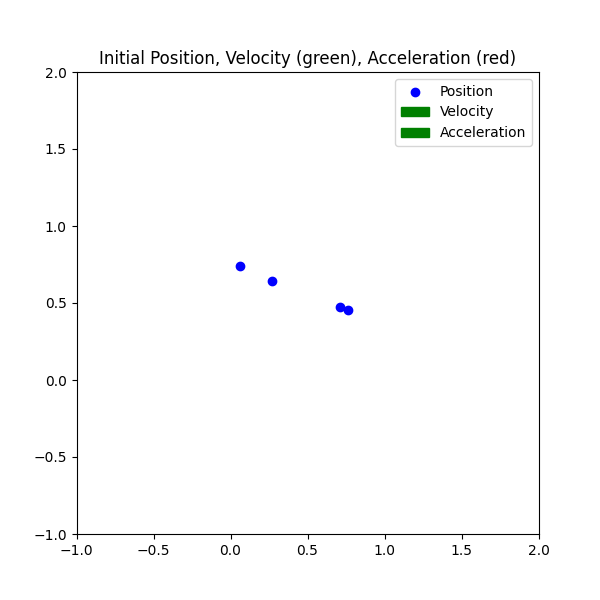
\includegraphics[width=0.9\textwidth]{fig/sample1/dd.png} % first figure itself
        \caption{sample1 randomly initial position}
        \label{fig:fig1}
    \end{minipage}\hfill
    \begin{minipage}{0.45\textwidth}
        \centering
        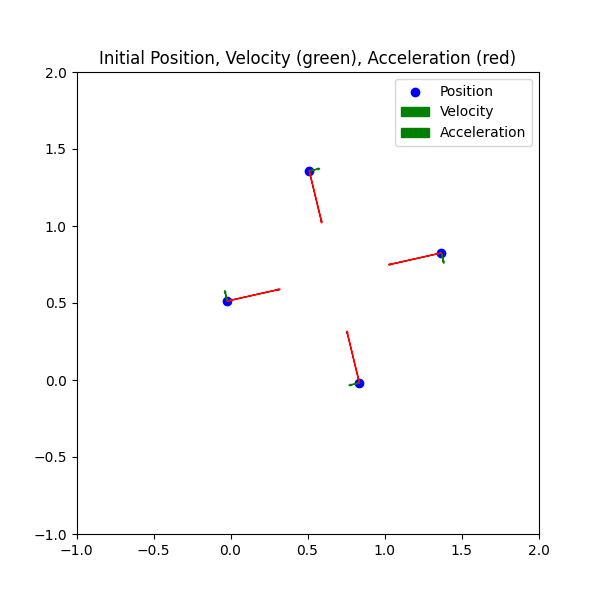
\includegraphics[width=0.9\textwidth]{fig/sample1/dd_18254.png} % second figure itself
        \caption{sample1 after a period of time}
    \end{minipage}
\end{figure}
\begin{figure}[ht!]
    \centering
    \begin{minipage}{0.45\textwidth}
        \centering
        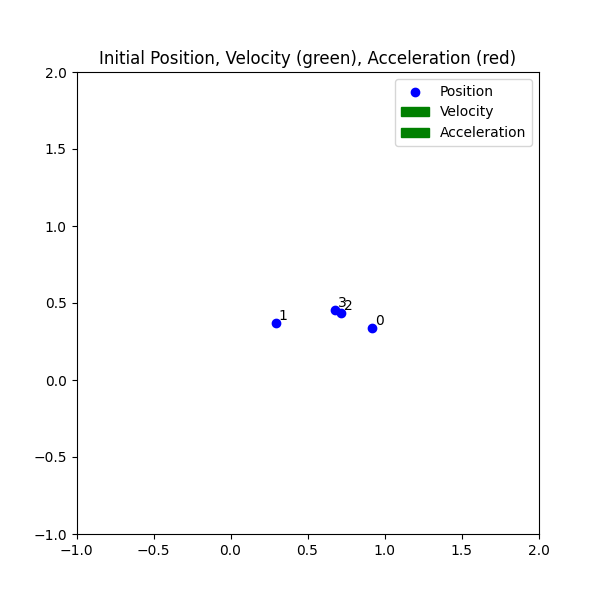
\includegraphics[width=0.9\textwidth]{fig/sample2/dd.png} % first figure itself
        \caption{sample1 randomly initial position}
        \label{fig:fig2}
    \end{minipage}\hfill
    \begin{minipage}{0.45\textwidth}
        \centering
        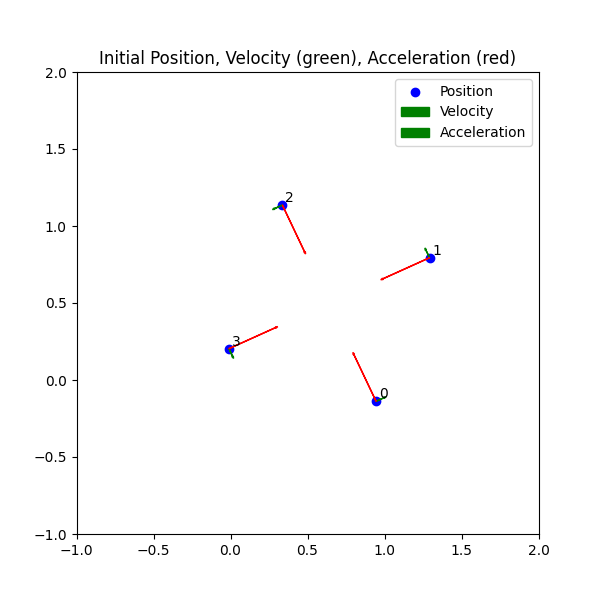
\includegraphics[width=0.9\textwidth]{fig/sample2/dd_18993.png} % second figure itself
        \caption{sample2 after a period of time}
    \end{minipage}
\end{figure}

\subsubsection{Ten drone case:derivation}
undergoing

\subsubsection{Ten drone case:result}
undergoing

\subsection{some analysis why it will have a stability property}
\subsubsection{the terminate radius R}
undergoing

\subsubsection{the terminate center O}
undergoing

\subsubsection{graph theory part}
The \(t(i)\) forms a graph which have \(n\) points
and \(n\) oriented edges, this forms a tree with a extra
edges, and this case It will obviously form a Unicyclic Graph.

Which is a tree if we treat all the point on the
loop as the same point.

\subsection{target distance method}
undergoing

\subsection{target distance method:simulation}
undergoing

\section{Zinan Su's approach}
\subsection{notations \& equations}
safe collide radius is \(d_s\)
\[
    \sigma=2d_s
\]
\(NUM\) is the total number of the drones.
And then we want the following dynamic system
\[\begin{bmatrix}
        \frac{d\vec{p_i}}{dt} \\
        \frac{d\vec{v_i}}{dt}
    \end{bmatrix}=
    \begin{bmatrix}
        \vec{v_i} \\
        \vec{a_i}
    \end{bmatrix}
\]
circle origin is a function
\[
    c=\frac{1}{NUM}\sum_{k=1}^{NUM}p_k
\]
Four constants.
\[
    k_p=
\]
\[
    k_d=
\]
\[
    k_v=
\]
\[
    k_r=
\]
\[
    R^*=\frac{1}{NUM}\sum_{k=1}^{NUM}p_k(0)-c(0)
\]
\[
    v_d=\frac{1}{NUM}\sum_{k=1}^{NUM}\|v_k(0)\|
\]
and
\[
    r_i=p_i-c
\]
\[
    d_i=\|r_i\|
\]
\[
    \hat{r_i}=\frac{r_i}{d_i}
\]
\[
    \hat{\theta_i}=\mathbb{M}_\theta r_i
\]
\[
    \mathbb{M}_\theta=
    \begin{bmatrix}
        0  & 1 \\
        -1 & 0
    \end{bmatrix}
\]
\[
    {v_{i}}_{\parallel}=\hat{r_i}\cdot v_i
\]
\[
    {v_{i}}_{\perp}=\hat{\theta_i}\cdot v_i
\]
\[
    U(r)=k_re^{-\frac{r}{2\sigma^2}}
\]
\[
    U_{ij}=U(\|p_i-p_j\|)
\]
\[
    \vec{u_i}_1=[-k_p(d_i-R^*)-k_d{v_{i}}_{\parallel}]\hat{r_i}
\]
\[
    \vec{u_i}_2=[-k_v({v_{i}}_{\perp}-v_d)]\hat{\theta_i}
\]
\[
    \vec{u_i}_3=\sum_{\forall k\neq i}(-\nabla_{p_i}U_{ij})
\]
\[
    \vec{u_i}=\vec{u_i}_1+\vec{u_i}_2+\vec{u_i}_3
\]




\bibliographystyle{plain}  % or another style like unsrt, IEEEtran, etc.
\bibliography{references}  % references.bib is the file name

\end{document}
